\documentclass[a4paper,twoside,titlepage,12pt]{article}
%
% Suomalaiset asetukset
\usepackage[finnish]{babel}
\usepackage[utf8]{inputenc}
\parindent0.0cm
\parskip0.23cm % Toista \tableofcontents:n jälkeen, muuten tulee harva sisällysluettelo
\frenchspacing
%
% Muita paketteja
\usepackage{listings}
\lstloadlanguages{SQL,Python}
\renewcommand{\lstlistingname}{Listaus}
\renewcommand{\lstlistlistingname}{Listaukset}

\usepackage{tikz}
\usepackage{graphicx}

% European Computer Modern fonts, scalable Type1 instead of bitmap fonts
\usepackage{ae}

%\pagestyle{headings}

%
% Hyperref pitää ladata viimeisenä
\usepackage{hyperref}

\begin{document}


%
% Etusivu
%
\begin{titlepage}

\vskip5.0cm

\begin{center}

{\huge
\vspace*{0.0cm}
\parskip1.0cm
\emph{Minivr}: junayhtiön tietojärjestelmä

Kurssin T-76.1143 harjoitustyö

{ \Large 5.11.2010 }

{ \Large Ryhmä 55: }

\large
Mikko Markus Torni $<$mtorni@cc.hut.fi$>$ (51161R) \\
    Sami J. Lehtinen $<$sjl@iki.fi$>$ (44814P) \\
    Matti Niemenmaa $<$mniemenm@cc.hut.fi$>$ (77243K)

}

\vskip5.0em

\vfill

\begin{flushleft}

\emph{Lähdekoodi:}

\indent \url{https://github.com/sjlehtin/minivr/}

\emph{Käyttöliittymädemo:} (tullaan vielä hiomaan)\\
\url{http://semeai.org:8000/}

\emph{Toteutusalusta:} Python + Django, PostgreSQL 8.0+

\emph{Demoajankohta:} 11.11. klo 15:20

\end{flushleft}

\end{center}


\end{titlepage}

\newpage

%
% Ensimmäinen sivu, sisällysluettelo
%

\parskip0.00cm % Ilman tätä tulee harva sisällysluettelo

\tableofcontents
\listoffigures
\lstlistoflistings

\parskip0.23cm % Vasta \tableofcontents:n jälkeen, muuten tulee harva sisällysluettelo

\newpage

%
% Ensimmäinen varsinainen tekstisivu
%

\section{Johdanto}

Teimme \href{http://www.aalto.fi/}{Aalto-yliopiston} \href{http://www.tkk.fi/}{Teknilliseen korkeakoulun} tiedonhallintajärjestelmät-kurssille (T-76.1143) vuoden 2010 syyslukukaudella harjoitustyön.



\subsection{Tehtävänanto: junayhtiön tietojärjestelmä}

Valitsimme kurssin T-76.1143 annetuista harjoitustyöaiheista junayhtiön tietojärjestelmän. Tehtävä oli annettu seuraavasti:

\begin{quotation}
\itshape
Asiakkaat voivat hakea palvelun kautta juna-aikatauluja, ja varata lippuja (jotka ovat haettavissa asemalta lähdettäessä), mikäli niitä on jäljellä. Lippujen hinnat riippuvat pääteasemista, junavuorosta sekä ostajan statuksesta (opiskelija/aikuinen jne.). Eri junavuoroilla on omat lähtö -ja päätepysäkit, eivätkä junavuorot välttämättä pysähdy kaikilla asemilla. Reitit haarautuvat rautatieverkostossa täysin mielivaltaisesti. Esimerkiksi pysäkiltä B voi olla kiskot pysäkeille A, C, D ja E, eikä ainoastaan "edelliselle pysäkille A ja seuraavalle pysäkille C". Järjestelmän tulisi pystyä näyttämään käyttälle reittioppaan tavoin eri vaihtoehdot matkustaa paikasta x paikkaan y, huomioiden mahdolliset vaihdot, sekä optimoiden ajankäytön ja hinnan.

Junavuoron voi olettaa kulkevan eri kausina (kesä/talvi) tietyn viikonpäivän tiettyyn kellonaikaan. Eri junavuorojen nopeuksista toisiinsa nähden ei voi tehdä mitään oletuksia.

Aihe tarjoaa paljon haastetta ja päänvaivaa erityisesti tietokannan rakenteen suunnittelussa. Haastetta voi kasvattaa entisestään esimerkiksi muuttamalla osan junavuoroista lähijuniksi, jolloin lippuja ei voi varata ennalta, ja hinnoittelu tapahtuu kuljettujen vyöhykkeiden perusteella. Toisaalta kaukojunien liput voisi pystyä varaamaan tietylle istumapaikalle tiettyyn vaunuluokkaan (travel/business).

Aiheeseen voi ottaa ideoita esim. VR:n sivuita.
\end{quotation}

\subsection{Järjestelmän vaatimukset}
Käyttäjät etsivät järjestelmää käyttäen itselleen sopivia junavuoroja.
Järjestelmän pitää pystyä hakemaan käyttäjälle reitti annettujen asemien
välille. Jos suoraa yhteyttä ei löydy, järjestelmä yrittää löytää käyttäjälle
mahdollisimman hyvän vaihtoyhteyden. Käyttäjän pitää pystyä varaamaan lippuja
valitsemalleen reitille.

\lstset{language=SQL}

\section{Tietokanta}

Valitsimme tietokannaksi vapaan PostgreSQL\footnote{\url{http://www.postgresql.org/}}-tietokannan. PostgreSQL on ohjelmistosuunnittelijaystävällinen sekä tarjoaa suorituskykyä ja joustavan indeksoinnin.

\subsection{ER-malli}

\begin{figure}
  \includegraphics[scale=0.5,angle=270]{relations}
  \caption{ER-malli keskeisimmista relaatioista}
\end{figure}

\textbf{TODO:} Kaavion sanallinen selvennys. Selittäkää ER-kaaviossa tehdyt ratkaisut, kaavion täytyy olla ulkopuolisen ymmärrettävissä.

\subsubsection{Connection}

Kuvaa raideyhteyttä kahden aseman välillä.
\begin{lstlisting}
INSERT INTO minivr_customertype
            (id, out_of_id, to_id, distance, cost)
     VALUES (0, 0, 1, 32, 26),
            (1, 1, 0, 32, 26),
            (2, 1, 2, 44, 39),
            (4, 2, 1, 44, 39)
\end{lstlisting}

\subsubsection{CustomerType}

Asiakastyyppi lipulle. Pääasiassa alennuslippujen määrittelyyn.
\begin{lstlisting}
INSERT INTO minivr_customertype
            (id, name)
     VALUES (1, 'Aikuinen'),
            (2, 'Opiskelija')
\end{lstlisting}

\subsubsection{Service}

Junavuoro, esimerkiksi \emph{IC2 109 1.12.2010 klo 12:15}. Sovellus tukee varauksia vain yhteen vuoroon kerrallaan eli päivittäin kulkevaan junaan ei voi varata paikkaa ylihuomiselle.
\begin{lstlisting}
INSERT INTO minivr_service
            (id, train_id, departure_time, free_seats)
     VALUES (0, 60, '12:15', 26),
            (1, 90, '13:50', 97)
\end{lstlisting}

\subsubsection{Station}

Asema, joilta junat voivat lähteä ja pysähtyä.
\begin{lstlisting}
INSERT INTO minivr_station
            (id, name)
     VALUES (0, 'Helsinki'),
            (1, 'Pasila'),
            (2, 'Tikkurila')
\end{lstlisting}

\subsubsection{Stop}

Yksittäinen pysähdys asemalla junavuorolle.
\begin{lstlisting}
INSERT INTO minivr_stop
            (id, service_id, station_id, arrival_time, departure_time, year_min, year_max, month_min, month_max, weekday_min, weekday_max)
     VALUES (0, 0,  25,NULL, 0,2010,2011,1,12,1,7),
            (1, 0,  28,  14,15,2010,2011,1,12,1,7)
\end{lstlisting}

\subsubsection{Ticket}

Vuorolle varattu lippu.
\begin{lstlisting}
INSERT INTO minivr_ticket
            (id, service_id, customer_type_id, price_per_cost)
     VALUES (0, 0, 1, 0.331600),
            (1, 1, 1, 0.859600)
            (2, 2, 1.613300)
\end{lstlisting}

\subsubsection{Train}

Juna, jolla vuoro ajetaan.
\begin{lstlisting}
INSERT INTO minivr_train
            (id, name, seats)
     VALUES (0, 'IC2 109', 120)
            (1, 'IC 11', 120)
            (2, 'IC 113', 84)
\end{lstlisting}


\subsection{Tietokantatoteutus}

Taulujen luontikomennot ovat listauksessa~\ref{lst:sqlcreatetables} sivulla~\pageref{lst:sqlcreatetables}. Tietokantataulut luotiin Djangon objekti-relaatiokuvausmoduulia käyttäen, joka loi SQL-taulut ja päivitti tietokantarakenteet kehityksen aikana.

Suoraviivaisesta ER-mallin muunnoksesta relaatiomalliksi täytyi poiketa monissa kohdissa johtuen käytetyn objekti-relaatiokuvaustekniikan rajoituksista. Tekniikka ei sallinut muunmuassa useamman attribuutin avaimia. Tietokantaan ei voinut myöskään laittaa kuin yksinkertaisia tarkistuksia tiedon oikeellisuudesta.

Käytetyn tekniikan rajoituksia olisi voinut osin kiertää käyttämällä tietokantapalvelimeen tallennettuja proseduureja tai näkymiä. Projektin yhteydessä haluttiin kuitenkin opetella objekti-relaatiokuvauksen käyttöä sen ketteryyden ja käytännöllisyyden vuoksi.

\subsubsection{Testidata}

Pohjana testidatalle on ote VR:n junavuorojen aikatauluista CSV\footnote{Comma Separated Values}-muodossa. Lähdekoodin tiedostossa \texttt{schedules.csv} on riveittäin lueteltu junavuoron tunnus, pysäkki, saapumisaika asemalle ja lähtöaika asemalta.

\begin{figure}
\begin{lstlisting}
IC2 109,Helsinki,,14:12
IC2 109,Pasila,14:17,14:18
IC2 109,Tikkurila,14:27,14:28
IC2 109,Lahti,15:06,15:08
IC2 109,Kouvola,15:40,
IC 11,Helsinki,,18:12
\end{lstlisting}
[\ldots]
  \caption{Ote junavuorojen testidatasta}
\end{figure}

Projektissa testidata generoidaan tietokantaan Python-skriptillä, joka luo tarvittavat tietorakenteet ja täydentää syöttötietoja satunnaisdatalla muunmuassa etäisyydet ja hinnat.

\subsubsection{Normalisointi}
\textbf{TODO:} Esitys funktionaalisista riippuvuuksista taulujen attribuuttien välillä. Ovatko taulut BCNF-normaalimuodossa? BCNF-normaalimuodon rikkominen edellyttää perustelut.

\subsubsection{Indeksointi}
Junayhteyksien haku on toteutettu Dijkstran algoritmilla sovelluksessa siten että tietokannalle tehdään tiheästi yksinkertaisia kyselyitä ja datamäärä on pieni. Indekseistä on rajoitetusti apua vain suuremmissa tauluissa joissa on yli tuhat riviä testidataa (\emph{Connection}, \emph{Stop}).

Tauluissa on indeksejä primääriavaimien lisäksi seuraavasti:

\begin{tabular}{ll}
\emph{Ticket} & service\_id, customer\_type\_id\\
\emph{Service} & train\_id\\
\emph{Stop} & service\_id, station\_id\\
\emph{Connection} & out\_of\_id, to\_id\\
\end{tabular}

\subsection{Tärkeimmät tietokantakyselyt}

\subsubsection{Junayhteyksien haku Dijkstran algoritmilla}
Toteutetun työn tärkein osuus on tarjota mahdollisia junayhteyksiä asiakkaalle. Tietokantaan on tallennettu saapumis- ja lähtöaikoja junavuoroittain. Ohjelman tehtävänä on päätellä kelvolliset suorat ja vaihdolliset junayhteydet ja esittää ne yksinkertaisessa muodossa.

Yksi mahdollinen tapa ratkaista ongelma on ajatella toteutuvia junavuoroja suunnattuna verkkona (jossa voi olla silmukoita). Ratkaisun voi löytää soveltamalla jotain tunnettua algoritmia polkujen löytämiseksi.

Toteutimme reittihakuihin muunnelman Dijkstran algoritmista\footnote{Katso algoritmin kuvaus esimerkiksi \href{http://fi.wikipedia/Dijkstran\_algoritmi}{Wikipediasta}} joka löytää vaihtoehtoiset reitit.

\lstset{language=SQL,caption=Esimerkki kyselylauseesta}
\begin{lstlisting}
SELECT * FROM
  (SELECT
     (60 * extract(hour   from minivr_service.departure_time)
       +   extract(minute from minivr_service.departure_time)
       + minivr_stop.departure_time
       - ?)
     AS t,
     minivr_stop.*
     FROM minivr_stop
         INNER JOIN minivr_service
                 ON (minivr_stop.service_id = minivr_service.id)
         INNER JOIN minivr_station
                 ON (minivr_stop.station_id = minivr_station.id)
     WHERE UPPER(minivr_station.name::text) = UPPER(?)
       AND minivr_service.free_seats > 0
       AND (minivr_stop.year_min IS NULL
            OR (    minivr_stop.year_min <= wanted_year
                AND minivr_stop.year_max >= wanted_year
                AND minivr_stop.month_min <= wanted_month
                AND minivr_stop.month_max >= wanted_month
                AND minivr_stop.weekday_min <= wanted_weekday
                AND minivr_stop.weekday_max >= wanted_weekday))
       AND minivr_stop.departure_time IS NOT NULL)
  AS ts
  ORDER BY ts.t - (24*60) * floor(ts.t / (24*60)) DESC)
\end{lstlisting}

\section{Käyttöliittymä}

Ryhmän jäsenten kiinnostuksen perusteella valitsimme käyttöliittymän toteutukseen \href{http://www.python.org/}{Python}-ohjelmointikielen\footnote{\url{http://www.python.org/}} ja Python-pohjaisen \href{http://www.djangoproject.com/}{Django-kehitysrungon}\footnote{\url{http://www.djangoproject.com/}}.

Django on korkean tason Web-kehitysympäristö joka kannustaa nopeaan kehitykseen ja puhtaaseen, pragmaattiseen suunnitteluun. Djangon ominaisuuksista käytimme objekti-relaatiokuvausta, jonka avulla ohjelmoidessa ei tarvitse erikseen työstää SQL-rajapinnan tietotyyppimuunnoksia.

Ohjelmistokehityksen apuna käytimme Djangon mukana tulevaa kehityswebbipalvelinta joka soveltuu hyvin prototyyppivaiheeseen.

Tässä osassa esittelemme käyttöliittymän keskeisimmät sivut ja toiminnallisuudet.

\subsection{Yleistä}
Käyttäjä voi useimmissa ruuduissa klikata junavuoron nimeä jolloin näkyviin tulee asemakohtaiset aikataulut, tai käyttää \emph{Varaa}-painiketta paikan varaamiseen junavuoroon.

\subsection{Reitin haku}
Sivulla käyttäjä voi hakea vuoroja asemalta mille tahansa muulle asemalle. Käyttäjän täytyy syöttää toivottu lähtö- tai saapumisaika. Haun tuloksena käyttäjälle näytetään kaikki mahdolliset junavuorot saman vuorokauden sisällä.

Haun suorittamisen jälkeen käyttäjällä on mahdollisuus varata paikka haluamaansa junavuoroon painamalla \emph{Varaa}-painiketta. Järjestelmä ilmoittaa onnistuiko varaus.

\begin{figure}
  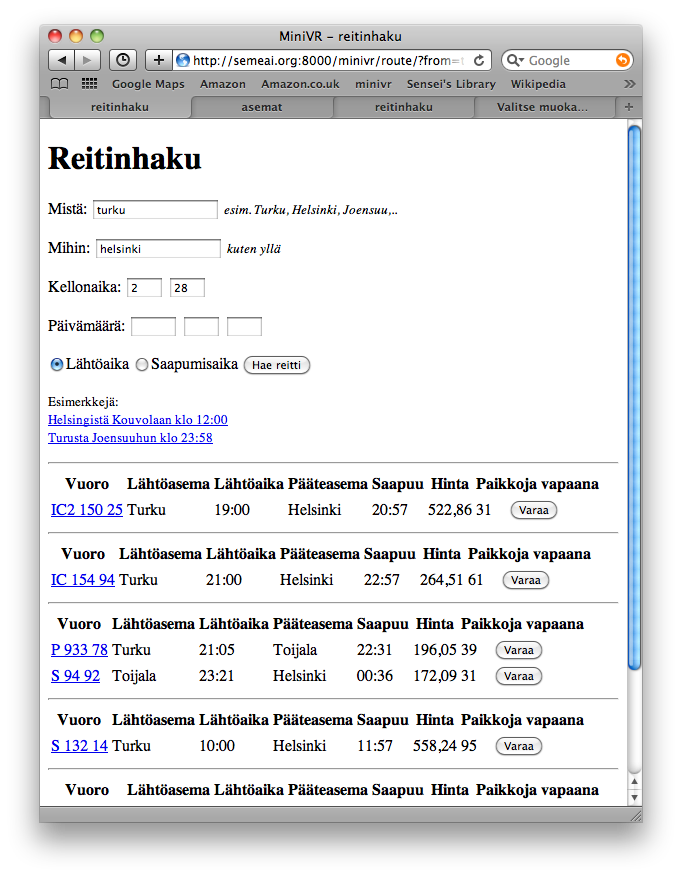
\includegraphics[width=130mm]{route.png}
  \caption{Reitin haku}
\end{figure}

\subsection{Kaikki asemat}
Sivulla näkyy lista kaikista asemista.

\subsection{Varauksen onnistuminen}

Reittihausta varauksen onnistuminen (tai epäonnistuminen) näytetään
käyttäjälle erillisellä sivulla.

Tältä sivulta pitäisi pystyä palaamaan rettihakusivulle (tämä on vielä
tekemättä).

\section{Viimeistely}

Ryhmällä on tarkoitus vielä lisätä lisätä linkkejä sivujen välille
käyttökokemuksen parantamiseksi (mm. varauksen vahvistussivulta takaisin
reittihakuun).

Virhesivuja ei ole viimeistelty (kaksi yhtäaikaista varausta viimeiseen
paikkaan, toinen siis epäonnistuu).

Reitinhaku sallii vaihdon junavuorosta toiseen kesken matkan, jos saapumis- ja
lähtöaikojen ero ylittää kovakoodatun rajan: 5 minuuttia. Demoon mennessä on
tarkoitus antaa käyttäjälle mahdollisuus valita tämä raja.

\section{Loppusanat}
\subsection{Työmäärä}
\textbf{TODO:} Matti Niemenmaan työtunnit

Mikko Markus Torni käytti harjoitustyöhön aikaa yhden tunnin ideoiden ylös kirjaamiseen, 12 tuntia dokumentoinnissa ja kaksi tuntia koodiin tutustumiseen.

Sami J. Lehtinen käytti 4 tuntia ylläpitotoimiin, 20 tuntia koodaamiseen
ja Djangoon tutustumiseen sekä 4 tuntia dokumentointiin.

\subsection{Oma arvio harjoitustyöstä}

Ryhmä aloitti työn tekemisen toden teolla aivan liian myöhään.

\subsection{Palaute kurssin järjestäjille}

Ei valittamista kurssijärjestelyistä.

%
% Liitteet
%
%
\newpage
\section*{Tietokannan luontikomennot}

\lstinputlisting[language=SQL,breaklines=true,breakatwhitespace=true,frame=single,basicstyle=\small,label=lst:sqlcreatetables,caption=Tietokantataulujen luontikomennot]{minivr.sql}

\end{document}
